\documentclass[a4paper,10pt]{article}
\usepackage[utf8]{inputenc}
\usepackage[T1]{fontenc}
\usepackage[left=0.8cm,right=0.8cm,top=0.8cm,bottom=0.8cm]{geometry}
\usepackage{enumitem}
\usepackage{titlesec}
\usepackage{parskip}
\usepackage{graphicx}
\usepackage{hyperref}
\usepackage{tikz}
\usepackage{adjustbox}
\usepackage{xcolor}
\usepackage[most]{tcolorbox}
\usepackage{pifont}
\definecolor{bleu}{HTML}{013c63}
\newcommand{\starfull}{\textcolor{bleu}{\ding{72}}}
\newcommand{\starempty}{\textcolor{bleu}{\ding{73}}}
\newcommand{\starhalf}{\textcolor{bleu}{\ding{74}}}
\newcommand{\cvtext}{\fontsize{8}{10}\selectfont}
\newcommand{\cvtextsmall}{\fontsize{7}{9}\selectfont}
\tcbset{
  cvbox/.style={
    colframe=bleu,
    colback=white,
    boxrule=0.4pt,
    arc=2pt,
    left=6pt,
    right=6pt,
    top=4pt,
    bottom=4pt,
    enhanced
  }
}
\titleformat{\section}{\Large\bfseries\color{bleu}}{}{0em}{}
\titleformat{\subsection}{\bfseries\color{bleu}}{}{0em}{}
\pagestyle{empty}
\hypersetup{
  pdfauthor={Victor Dauphin},
  pdftitle={CV Victor Dauphin},
  pdfsubject={CV},
  pdfproducer={LaTeX},
  pdfcreator={pdflatex},
  colorlinks=true,
  urlcolor=bleu,
  linkcolor=bleu,
  citecolor=bleu
}
\begin{document}
\noindent
\begin{minipage}[t]{0.72\textwidth}
  {\LARGE \textcolor{bleu}{\textbf{Technical Mentor - Fullstack Java / Angular Dev}}}\\[0.5em]
  {\LARGE \textcolor{bleu}{\textbf{Victor Dauphin}}}\\[0.5em]
  Metz • 37 years old • Driver's License B \\  
  \href{mailto:victor.dauph@gmail.com}{victor.dauph@gmail.com} • +33 6 95 19 99 40 \\  
  \href{https://github.com/VictorDauph}{GitHub} •  
  \href{https://linkedin.com/in/victor-dauphin-83430840}{LinkedIn}\\
\end{minipage}
\hfill
\begin{minipage}[t]{0.25\textwidth}
  \begin{flushright}
  \raisebox{-2.6cm}{
    \begin{tikzpicture}
      \draw[fill=white, draw=bleu, line width=1pt] (0,0) circle (1.51cm);
      \clip (0,0) circle (1.5cm);
      \node at (0,0) {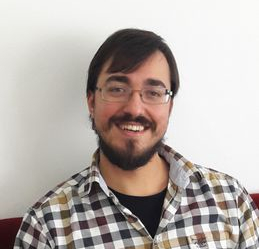
\includegraphics[width=3cm]{images/photo.jpg}};
    \end{tikzpicture}
    }
  \end{flushright}
\end{minipage}
\vspace{1.5em}
\noindent
\begin{minipage}[t]{0.3\textwidth}
  \section*{Skills}
  \begin{tcolorbox}[cvbox, width=\linewidth]
      \subsection*{Core stack}
      {\normalsize
      Java / Spring Boot \\
      Angular / TypeScript \\
      PostgreSQL
      } \\
      \subsection*{Additional technologies}
      {\normalsize
      Node.js / Express / NestJS \\
      Vue.js \\
      MongoDB \\
      NiFi \\
      PHP / Dolibarr
      } \\
      \subsection*{DevOps \& Quality}
      {\normalsize
      Docker \\
      GitLab CI \\
      Unit testing: JUnit \\
      SonarQube / ESLint
      } \\
      \subsection*{Best practices}
      {\normalsize
      Clean Code \\
      SOLID \\
      CI/CD \\
      OWASP \\
      WCAG \\
      Git workflow
      }
  \end{tcolorbox}
  \section*{Certifications}
  \begin{tcolorbox}[cvbox, width=\linewidth]
    \begin{itemize}[leftmargin=*]
      \item AWS Cloud Practitioner (2023)
      \item DevSecOps Foundation (2023)
      \item 2AIConcept Expert Trainer (2024)
    \end{itemize}
  \end{tcolorbox}
  \section*{Education}
  \begin{tcolorbox}[cvbox, width=\linewidth]
    \begin{itemize}[leftmargin=*]
      \item M2i \textit{POEI Fullstack Spring/Angular} (2022)
      \item OpenClassrooms \textit{Fullstack Node/React} (2021)
      \item ENSGSI \textit{General Engineer} (2013)
    \end{itemize}
  \end{tcolorbox}
\end{minipage}
\hfill
\begin{minipage}[t]{0.68\textwidth}
\section*{Profile}
  Fullstack Java / Angular developer with 4 years of experience in corporate environments.  
  I design robust applications with a focus on code quality, CI/CD and engineering best practices.  
  I also support teams in project structuring and technical upskilling.\\

\section*{Professional Experience}
  \begin{tcolorbox}[cvbox, width=\linewidth,fontupper=\cvtext]
  \subsection*{Web Development Trainer -- freelance} \textit{Oct 2024 -- Present}
  \begin{itemize}[leftmargin=*]
    \item Java new features (v6 to v21).
    \item Modern HTML5 and CSS3. development
    \item Angular: architecture, components, services, RxJS, Reactive Forms.
    \item Introduction to SQL/PostgreSQL.
    \item PL/SQL: stored procedures, functions, triggers in an Oracle database.
  \end{itemize}
  \subsection*{Freelance Developer -- Arterrien \textit{PHP / Dolibarr}} \textit{Apr 2025 -- Jun 2025}
  \begin{itemize}[leftmargin=*]
  \item Continuous improvement of a custom ERP module based on Dolibarr.
  \item Integration of PHPStan (level 4) with custom stubs for the Dolibarr context.
  \item Setup of a Dockerized CI/CD runner (Google Cloud VM + GitLab).
  \item Implementation of unit tests with PHPUnit.
  \end{itemize}
  \subsection*{Trainer Certified Fullstack Developer \textit{Express / Angular}} \textit{Nov 2024 -- Apr 2025}
  \begin{itemize}[leftmargin=*]
    \item Intensive training for job seekers.
    \item Hands-on projects: Angular, Express, MongoDB, SQL.
    \item Docker, Git, CI/CD, automated testing.
  \end{itemize}
  \subsection*{Fullstack Developer -- Davidson \textit{Vue / NestJS}} \textit{Jun 2024 -- Sept 2024}
  \begin{itemize}[leftmargin=*]
    \item Refactored Vue Router, implemented todo/notifications modules.
    \item Peer reviews, documentation, production deployment.
  \end{itemize}
  \subsection*{NiFi / Java Developer -- Atos / EDF \textit{NiFi / Java / VBA}} \textit{Sept 2023 -- Jun 2024}
  \begin{itemize}[leftmargin=*]
    \item Designed and developed data flows with Apache NiFi.
    \item Created a custom NiFi processor in Java to meet specific business needs.
    \item Automated tasks with Excel macros (VBA) and wrote tests with Unifier.
  \end{itemize}
  \subsection*{Fullstack Developer -- Atos / Agirc-Arrco / CEA \textit{Angular / Java SpringBoot}} \textit{Oct 2022 -- Jun 2023}
  \begin{itemize}[leftmargin=*]
    \item Developed user interfaces in Angular, integrated with REST APIs.
    \item Designed backend services with Spring Boot and managed data with PostgreSQL.
    \item Wrote unit tests with JUnit to ensure code reliability.
    \item Involved in the entire project cycle: analysis, development, testing, and delivery in an agile environment.
  \end{itemize}
\end{tcolorbox}

\section*{Other Professional Experience}
\begin{tcolorbox}[cvbox, width=\linewidth,fontupper=\cvtextsmall]
  \begin{itemize}[leftmargin=*]
    \item \textbf{Freelance Trainer} – Interpersonal Communication (2018–2020)  
    Led dynamic training sessions based on improvisational theater.

    \item \textbf{Project Manager} – Sustainable Logistics (2017–2018)  
    Promoted eco-friendly solutions within a logistics cluster.

    \item \textbf{Project Leader} – Medical Logistics (2016–2017)  
    Coordinated teams and managed workflows for clinical research.

    \item \textbf{Co-founder} – Digital Startup (2013–2015)  
    Product development, team management, business strategy.
  \end{itemize}
\end{tcolorbox}
\end{minipage}
\end{document}
